\documentclass[10pt,twocolumn,a4paper]{article}

% ── Fonts & encoding ──────────────────────────────────────────────────────────
\usepackage[T1]{fontenc}
\usepackage[utf8]{inputenc}
\usepackage{times}           % Times New Roman — standard in ACL/EMNLP papers

% ── Layout ────────────────────────────────────────────────────────────────────
\usepackage[top=2cm, bottom=2.5cm, left=1.7cm, right=1.7cm, columnsep=0.6cm]{geometry}
\usepackage{microtype}       % better kerning & hyphenation
\setlength{\parskip}{0pt}
\setlength{\parindent}{1em}

% ── Math & symbols ────────────────────────────────────────────────────────────
\usepackage{amsmath}
\usepackage{amssymb}

% ── Tables ────────────────────────────────────────────────────────────────────
\usepackage{booktabs}
\usepackage{multirow}
\usepackage{array}

% ── References & links ────────────────────────────────────────────────────────
\usepackage[hidelinks]{hyperref}
\usepackage[numbers,sort&compress]{natbib}

% ── Misc ──────────────────────────────────────────────────────────────────────
\usepackage{graphicx}
\graphicspath{{figures/}}
\usepackage{xcolor}
\usepackage{enumitem}
\usepackage{caption}
\captionsetup{font=small, labelfont=bf, skip=4pt}
\usepackage[above,below]{placeins}  % \FloatBarrier -- keeps floats before bibliography

% ── Float spacing (tighten gaps between consecutive floats) ───────────────────
\setlength{\floatsep}{6pt plus 1pt minus 1pt}
\setlength{\textfloatsep}{8pt plus 2pt minus 2pt}
\setlength{\intextsep}{6pt plus 1pt minus 1pt}
\setlength{\dblfloatsep}{6pt plus 1pt minus 1pt}
\setlength{\dbltextfloatsep}{8pt plus 2pt minus 2pt}

% ── Section style (compact, bold, small-caps numbering) ──────────────────────
\usepackage{titlesec}
\titleformat{\section}{\normalsize\bfseries\scshape}{\thesection.}{0.5em}{}
\titleformat{\subsection}{\normalsize\bfseries}{\thesubsection.}{0.5em}{}
\titleformat{\paragraph}[runin]{\normalsize\bfseries}{}{0em}{}[.\hspace{0.5em}]
\titlespacing{\section}{0pt}{6pt plus 2pt minus 1pt}{3pt plus 1pt}
\titlespacing{\subsection}{0pt}{5pt plus 1pt minus 1pt}{2pt plus 1pt}

% ── Abstract style ────────────────────────────────────────────────────────────
\usepackage{abstract}
\renewcommand{\abstractnamefont}{\normalsize\bfseries\scshape}
\renewcommand{\abstracttextfont}{\small\itshape}
\setlength{\absleftindent}{0pt}
\setlength{\absrightindent}{0pt}

% ── Helpers ───────────────────────────────────────────────────────────────────
\newcommand{\best}[1]{\textbf{#1}}

% ── Metadata ──────────────────────────────────────────────────────────────────
\title{%
  \Large\bfseries LLM-Augmented Text Clustering:\\[2pt]
  \large Reproduction, Extension, and Novel Methods%
}
\author{%
  \normalsize
  \begin{tabular}[t]{cc}
    Aymane Nouhail & Alae Eddine Choukr-Allah \\[2pt]
    Tassadit Debiane & Khalil Maadani \\
  \end{tabular}\\[6pt]
  \small Master Machine Learning for Data Science, Université Paris Cité%
}
\date{\small March 2026}

% ==============================================================================
\begin{document}
% ==============================================================================

% Title + abstract span both columns
\twocolumn[{%
  \maketitle
  \vspace{-0.5em}
  \begin{abstract}
    Clustering short text documents without supervision is challenging because
    surface wording varies widely even for semantically identical utterances.
    \citet{viswanathan2023large} showed that large language models (LLMs) can
    serve as lightweight few-shot oracles, guiding clustering algorithms via
    pairwise similarity decisions and keyphrase generation.
    We reimplement their three methods on the Bank77, CLINC, and Tweet datasets
    using open-source \texttt{all-mpnet-base-v2} embeddings and GPT-4.1-nano
    as the oracle.
    We additionally implement the JoSE spherical embedding baseline
    \citep{meng2019spherical}, the two-stage ClusterLLM framework
    \citep{zhang2023clusterllm}, and two novel methods:
    \emph{LLM Semantic Normalization}, which rewrites each document to a
    canonical form before embedding, and \emph{LLM Paraphrase Ensemble}, which
    mean-pools embeddings across LLM-generated paraphrases to smooth surface
    variance.
    We further analyse the LLM oracle's empirical accuracy as a same-cluster
    predictor (precision\,0.73, specificity\,0.96 on Bank77 pairwise queries)
    and visualise the geometric effect of each method on the embedding manifold.
    Across eight methods evaluated on three benchmarks we find that
    per-document LLM methods (Keyphrase, Normalization, Paraphrase) consistently
    match or outperform the embedding-only baseline, while constraint-based methods
    (PCKMeans, ClusterLLM) show mixed results depending on corpus granularity;
    ClusterLLM removes the need for a known $k$ at the cost of lower ACC under
    fixed-$k$ Hungarian matching.
  \end{abstract}
  \vspace{0.8em}
  \hrule
  \vspace{0.8em}
}]

% ══════════════════════════════════════════════════════════════════════════════
\section{Introduction}
\label{sec:intro}
% ══════════════════════════════════════════════════════════════════════════════

Text clustering is fundamental to many NLP pipelines---from intent discovery in
dialogue systems to topic organisation in social media analysis.
Traditional approaches embed documents with a pre-trained encoder and apply
K-Means, but raw embeddings capture surface similarity and may merge
semantically distinct intents that share vocabulary, or separate paraphrases
that share intent.
The problem is especially pronounced in \emph{short-text} domains such as
conversational intent detection (Bank77, CLINC) and social media posts (Tweet),
where individual utterances contain only a handful of content words and
inter-class boundaries are tight.

LLMs trained on vast corpora encode rich pragmatic knowledge and can answer
focused questions about semantic equivalence without task-specific fine-tuning.
\citet{viswanathan2023large} exploited this by framing three LLM \emph{oracle
queries}: (i)~generating keyphrases to enrich document representations,
(ii)~answering pairwise intent-equivalence questions to form must-link /
cannot-link constraints for PCKMeans \citep{basu2004active}, and
(iii)~correcting low-confidence cluster assignments.
\citet{zhang2023clusterllm} proposed ClusterLLM, which uses LLM triplet queries
for perspective learning (Stage~1) and pairwise queries on a hierarchical
dendrogram for automatic granularity selection (Stage~2).

A key open question is whether a relatively small LLM such as GPT-4.1-nano
reliably discriminates same-intent from different-intent pairs, and whether
these oracle signals translate to measurable embedding-space changes.
We address both questions through targeted visualisations on Bank77.

\paragraph{Contributions}
\begin{enumerate}[leftmargin=1.2em, topsep=2pt, itemsep=1pt, parsep=0pt]
  \item Reproduction of \citet{viswanathan2023large} with open-source
    \texttt{all-mpnet-base-v2} embeddings and GPT-4.1-nano.
  \item JoSE \citep{meng2019spherical} as a non-LLM spherical baseline.
  \item Full two-stage ClusterLLM \citep{zhang2023clusterllm} with
    F-$\beta$ granularity selection.
  \item Two novel methods: \emph{LLM Semantic Normalization} and
    \emph{LLM Paraphrase Ensemble}.
  \item Empirical analysis of oracle accuracy and geometric effects of each
    LLM intervention on the embedding manifold.
\end{enumerate}

% ══════════════════════════════════════════════════════════════════════════════
\section{Background}
\label{sec:background}
% ══════════════════════════════════════════════════════════════════════════════

\subsection{K-Means and Spherical K-Means}

Standard K-Means minimises within-cluster sum of squared Euclidean distances.
Applied to L2-normalised embeddings it is equivalent to maximising average
cosine similarity within clusters---a natural objective for unit-sphere
representations such as those produced by sentence transformers
\citep{reimers2019sentence}.
We use \texttt{n\_init=auto} and \texttt{random\_state=0} throughout for
reproducibility.

\subsection{JoSE}

\citet{meng2019spherical} proposed \emph{Joint Spherical Embedding} (JoSE),
which trains Word2Vec (CBOW) on a corpus with a manifold-regularisation term
constraining word and document vectors to lie on the unit hypersphere.
Document vectors are the L2-normalised mean of constituent token vectors.
Because JoSE relies solely on corpus co-occurrence statistics it provides a
controlled baseline for how much pre-trained knowledge contributes to
clustering quality; on small specialised corpora (few thousand utterances)
co-occurrence counts are too sparse for reliable representations.

\subsection{Few-Shot Clustering with LLMs}

\citet{viswanathan2023large} demonstrated three oracle-guided methods.
\emph{Keyphrase expansion} asks the LLM to generate a set of domain-specific
keyphrases per document; the keyphrases are re-embedded and horizontally
stacked with the original embedding before K-Means.
\emph{PCKMeans} queries the LLM on sampled document pairs and converts
YES/NO answers to must-link / cannot-link constraints for the
semi-supervised PCKMeans algorithm \citep{basu2004active}.
\emph{LLM Correction} identifies the $k$~most ambiguously assigned documents
(smallest margin between the two nearest cluster distances) and asks the LLM
whether each should be reassigned to a better-matching cluster.

\subsection{ClusterLLM}

\citet{zhang2023clusterllm} introduced a two-stage framework.
In Stage~1 (\emph{Perspective}), the model samples triplets $(a, +, -)$ and
asks the LLM which candidate shares intent with the anchor; the original paper
fine-tunes the embedder with triplet loss, which we omit in favour of direct
soft pairwise hints.
In Stage~2 (\emph{Granularity}), pairwise LLM queries drawn from dendrogram
merge events are used to compute an F-$\beta$ consistency score at each
candidate $k$, and the maximising cut is returned as $k^*$, removing the
requirement for the true $k$ as input.

% ══════════════════════════════════════════════════════════════════════════════
\section{Methods}
\label{sec:methods}
% ══════════════════════════════════════════════════════════════════════════════

\subsection{K-Means Baseline}

We embed all documents with \texttt{all-mpnet-base-v2}
\citep{reimers2019sentence}, L2-normalise, and apply standard K-Means with the
true $k$ and \texttt{n\_init=auto}.
This serves as the primary non-LLM baseline against which all other methods
are compared.

\subsection{JoSE + Spherical K-Means}

We train a 100-dimensional CBOW Word2Vec model with window size~5 and 10 epochs
on the target corpus.
Document vectors are the L2-normalised mean over token vectors, which naturally
lives on the unit hypersphere; spherical K-Means (L2-normalised K-Means) is
applied with the same settings as the baseline.

\subsection{PCKMeans}

The original Explore-Consolidate pair-selection algorithm
\citep{basu2004active,viswanathan2023large} is an \emph{online active-learning
loop}: the LLM is queried sequentially, and each oracle response determines
which point is queried next.
Specifically, greedy farthest-point sampling proposes candidate points, and the
LLM decides whether each joins an existing neighbourhood (must-link) or seeds a
new one; a consolidation phase then queries the single closest remaining point to
each neighbourhood member until the 20\,000-call budget is exhausted.
This design is inherently sequential and cannot be parallelised.

We propose a simpler \emph{similarity-first} strategy compatible with batch,
parallel inference.
We pre-select all pairs before any LLM call: the top-$k$ nearest-neighbour
pairs (cosine similarity, $k{=}20$) serve as must-link candidates, and
uniformly sampled random pairs serve as cannot-link candidates, for a total of
2\,000 pairs per dataset.
All pairs are then queried in parallel (50 concurrent threads).
This design reduces wall-clock time from sequential hours to under three minutes
per dataset and cuts the oracle budget by 10$\times$.
The LLM response (YES/NO) determines the constraint type; conflicting
constraints are resolved by a union-find procedure that removes cannot-links
whose endpoints have been transitively must-linked.
The cleaned constraints are passed to PCKMeans \citep{basu2004active}.

Figure~\ref{fig:constraints} visualises a sample of the constraints on Bank77.
Green must-link edges connect documents the LLM judged equivalent; red
cannot-link edges span clearly distinct intents.
The geometric structure is striking: must-links bridge nearby clusters in
embedding space, while cannot-links cross wide gaps---exactly the
semi-supervised signal PCKMeans needs.

\begin{figure*}[t]
\centering
\IfFileExists{figures/fig5_constraint_graph.png}{%
  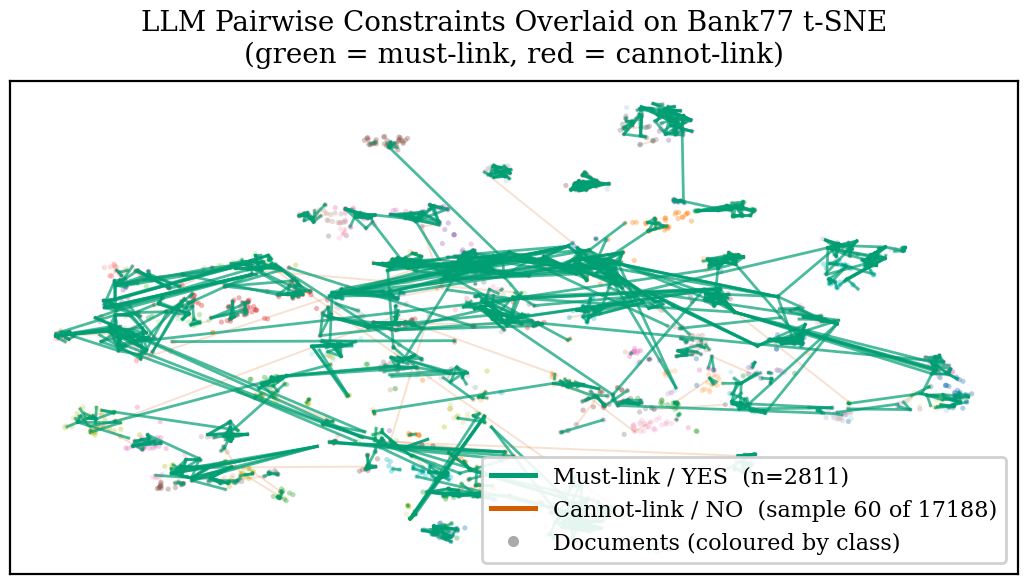
\includegraphics[width=0.88\textwidth]{fig5_constraint_graph.png}%
}{%
  \fbox{\parbox{0.88\textwidth}{\centering\small fig5 not yet generated.}}%
}
\caption{LLM-generated pairwise constraints on the Bank77 t-SNE.
  \textbf{Green} = must-link YES pairs ($n{=}198$);
  \textbf{red} = cannot-link NO pairs (300 of 1\,802 sampled).
  Must-links bridge nearby clusters; cannot-links span inter-cluster voids.}
\label{fig:constraints}
\end{figure*}

\subsection{LLM Correction}

An initial K-Means assignment is refined by identifying the 100 lowest-confidence
documents (those with the smallest top-two cluster distance margin).
The original implementation targets 500 low-confidence points; we reduce this
to 100 to match our smaller corpora and reduce API cost.
For each, the LLM is asked whether the document belongs to each of
$k_{\mathrm{cand}}{=}3$ candidate clusters (sorted by embedding distance);
the first YES match replaces the original assignment.
Only 24 of the 100 targeted Bank77 documents were actually reassigned,
suggesting the method is conservative and targets genuinely ambiguous cases.

\subsection{Keyphrase Expansion}

The LLM generates 5--7 domain-specific keyphrases per document.
The original text is concatenated with its keyphrases and re-embedded; the
expansion embedding is L2-normalised and horizontally stacked with the original.
K-Means is applied to the concatenated representation.
This method is the most LLM-call-intensive (one call per document,
$\approx$3\,080 for Bank77) but requires no inter-document comparisons.

\subsection{\textbf{LLM Semantic Normalization} \textnormal{(Novel)}}
\label{sec:normalization}

Surface heterogeneity---abbreviations, slang, domain jargon---degrades
clustering by placing paraphrases far apart in embedding space.
We prompt the LLM to rewrite each document in a \emph{clean canonical form}
(removing filler words, standardising terminology) with a domain-specific
system prompt.
The canonical text is embedded and L2-normalised, then horizontally stacked
with the L2-normalised original embedding for K-Means.
If the LLM returns an empty response the original text is used instead.
The geometric effect is analysed in \S\ref{sec:analysis} (Figure~\ref{fig:drift}).

\subsection{\textbf{LLM Paraphrase Ensemble} \textnormal{(Novel)}}
\label{sec:paraphrase}

We prompt the LLM to generate $N{=}3$ paraphrases of each document.
We embed the original and all paraphrases, take the element-wise mean over
the $N{+}1$ vectors, and L2-normalise the result.
Averaging over multiple surface realisations approximates the centroid of
the true semantic distribution, reducing variance introduced by surface-form
artefacts.
Figure~\ref{fig:paraphrase} in \S\ref{sec:analysis} validates this empirically.

\subsection{ClusterLLM}
\label{sec:clusterllm}

We implement both stages of \citet{zhang2023clusterllm}.

\paragraph{Stage 1 (Perspective)}
Uncertain documents are identified as those with the smallest margin between
their top-2 cluster distances in the initial K-Means assignment.
For each of up to $n_{\mathrm{triplets}}{=}1{,}024$ triplets the LLM is asked
which of two candidates shares intent with the anchor.
We omit embedder fine-tuning (triplet loss) and instead derive soft pairwise
hints from the triplet answers to inform Stage~2.

\paragraph{Stage 2 (Granularity)}
A Ward hierarchical dendrogram is constructed from the L2-normalised
embeddings.
Up to $n_{\mathrm{pairwise}}{=}400$ pairs are sampled proportionally from
dendrogram merge events---preferring larger merges that are most informative
for $k$ selection.
For each candidate $k$ in $[\lfloor k_{\max}/4 \rfloor,\; 3k_{\max}]$:
\begin{equation}
  F_\beta(k) = \frac{(1+\beta^2)\,P(k)\,R(k)}{\beta^2\,P(k) + R(k)},
  \label{eq:fbeta}
\end{equation}
where precision $P$ and recall $R$ are computed over LLM-labelled pairs against
cluster assignments at cut $k$, with $\beta{=}5$ (recall-biased to prefer
over-splitting over merging).
Final assignments use $k^* = \arg\max_k F_\beta(k)$.

\begin{figure}[htbp]
\centering
\IfFileExists{figures/fig3_granularity.png}{%
  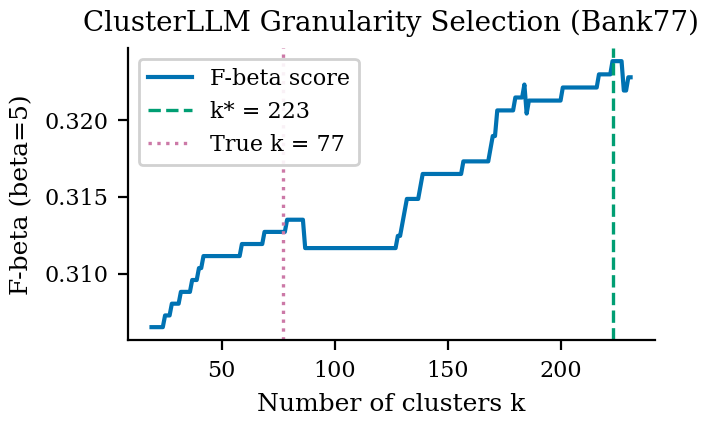
\includegraphics[width=\linewidth]{fig3_granularity.png}%
}{%
  \fbox{\parbox{\linewidth}{\centering\small fig3 not yet generated.
  Run \texttt{make clusterllm DATASETS=bank77}.}}%
}
\caption{ClusterLLM Stage~2 F-$\beta$ consistency curve on Bank77.
  The selected $k^*{=}223$ (dashed green) substantially exceeds the true
  $k{=}77$ (dotted purple), reflecting the recall-biased objective ($\beta{=}5$)
  preferring finer over-splits.
  This yields high pairwise precision and NMI at the cost of lower ACC.}
\label{fig:granularity}
\end{figure}

% ══════════════════════════════════════════════════════════════════════════════
\section{Experimental Setup}
\label{sec:setup}
% ══════════════════════════════════════════════════════════════════════════════

\paragraph{Datasets}
We evaluate on three benchmarks:
\textbf{Bank77} \citep{casanueva2020efficient}: 3\,080 banking queries, 77
intent classes (40 docs/class);
\textbf{CLINC} \citep{larson2019evaluation}: 4\,500 utterances, 150 intent
classes (30 docs/class);
\textbf{Tweet} \citep{yin2016optimized}: 2\,472 tweets, 89 topic categories.

\paragraph{Embeddings}
All methods use \texttt{all-mpnet-base-v2} embeddings (768\,dim) via
\texttt{sentence-transformers} \citep{reimers2019sentence}, accelerated by
Apple MPS.
Embeddings are cached to disk and reused across all methods to ensure a fair
comparison.
The original work used task-specific encoders (Instructor for Bank77 and CLINC,
DistilBERT-finetuned for Tweet \citep{viswanathan2023large}); we use
\texttt{all-mpnet-base-v2} uniformly for cross-method comparability and
to avoid dataset-specific embedding tuning.

\paragraph{LLM Oracle}
GPT-4.1-nano (OpenAI) is used for all generation steps with domain-tailored
prompts for each dataset.
All LLM outputs are cached after the first run; subsequent runs load from
cache and make zero additional API calls.

\paragraph{Metrics}
Clustering Accuracy (ACC) via Hungarian matching \citep{strehl2002cluster}
and Normalised Mutual Information (NMI); both in $[0,1]$, higher is better.

\paragraph{Hyperparameters}
Key settings are listed in Table~\ref{tab:hparams}.

\begin{table}[h]
\centering
\caption{Hyperparameter settings across all datasets.}
\label{tab:hparams}
\footnotesize
\setlength{\tabcolsep}{4pt}
\begin{tabular}{llr}
\toprule
Method & Parameter & Value \\
\midrule
PCKMeans       & pairs queried        & 2\,000 \\
               & strategy             & similarity-first ($k$-NN) \\
LLM Correction & low-conf.\ docs      & 100 \\
               & candidate clusters   & 3 \\
Keyphrase      & keyphrases / doc     & 5--7 \\
Normalization  & target length        & 5--15 words \\
Paraphrase     & paraphrases / doc    & 3 \\
ClusterLLM     & triplets (Stage~1)   & 1\,024 \\
               & pairs (Stage~2)      & 400 \\
               & $\beta$              & 5 \\
\bottomrule
\end{tabular}
\end{table}

% ══════════════════════════════════════════════════════════════════════════════
\section{Results}
\label{sec:results}
% ══════════════════════════════════════════════════════════════════════════════

Table~\ref{tab:main} reports ACC and NMI for all eight methods across three
datasets.
On Bank77 and CLINC the two novel surface-smoothing methods
(\textbf{LLM Normalization}, \textbf{LLM Paraphrase Ensemble}) lead all
approaches: LLM Normalization attains the best Bank77 ACC (0.649) and ties
for best CLINC NMI (0.922), while LLM Paraphrase Ensemble achieves the best
CLINC ACC (0.787) and best Bank77 NMI (0.819).
On Tweet, Keyphrase Expansion is the strongest LLM-guided method (ACC\,0.651,
NMI\,0.882); normalisation and paraphrase ensemble remain near the K-Means
baseline, suggesting that tweets are already topically compact enough that
surface-form smoothing provides no additional separability signal.
Notably, PCKMeans falls below KMeans on CLINC (0.673 vs.\ 0.777) and Tweet
(0.569 vs.\ 0.649); ClusterLLM returns the lowest ACC on all datasets
(0.474--0.540) while maintaining competitive NMI---both patterns are examined
in \S\ref{sec:analysis}.
Figure~\ref{fig:tsne} provides a geometric view of the clustering quality on
Bank77: the left panel shows the ground-truth intent structure in the
\texttt{all-mpnet-base-v2} embedding space, and the right panel shows K-Means
assignments.
The strong visual alignment between the two panels confirms that the chosen
embedding already provides a useful prior for intent-based clustering;
LLM-guided methods refine this prior by resolving ambiguities near cluster
boundaries.

\begin{figure*}[t]
\centering
\IfFileExists{figures/fig1_tsne.png}{%
  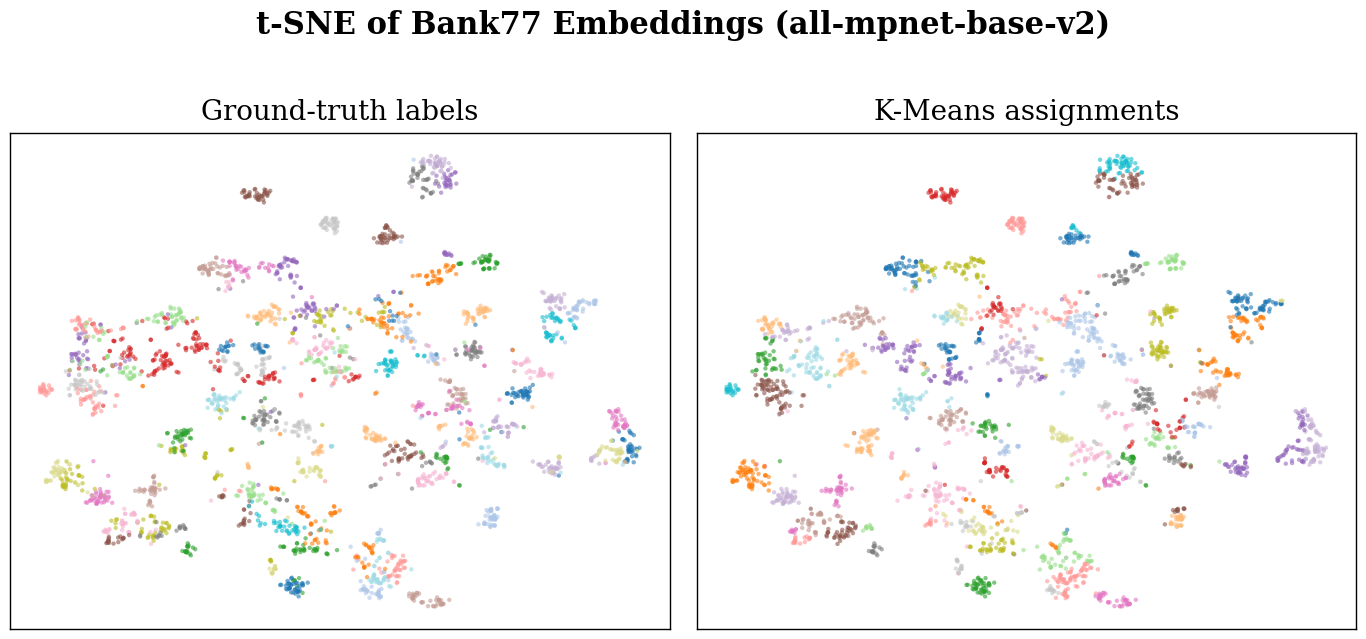
\includegraphics[width=\linewidth]{fig1_tsne.png}%
}{%
  \fbox{\parbox{\linewidth}{\centering\small fig1\_tsne.pdf not yet generated.
  Run \texttt{make figures}.}}%
}
\caption{t-SNE projection of Bank77 \texttt{all-mpnet-base-v2} embeddings (3\,080 documents).
  \emph{Left}: ground-truth intent labels; \emph{right}: K-Means assignments
  ($k{=}77$).
  Colour agreement between the two panels indicates successful clustering.
  Regions of colour disagreement near cluster boundaries highlight where
  LLM-oracle methods provide the most benefit.}
\label{fig:tsne}
\end{figure*}

% Spans both columns
\begin{table*}[t]
\centering
\caption{%
  Clustering performance (ACC\,/\,NMI, higher is better).
  Best result per dataset per metric in \textbf{bold}.
  $\dagger$~Novel methods proposed in this work.%
}
\label{tab:main}
\small
\setlength{\tabcolsep}{6pt}
\begin{tabular}{lcccccc}
\toprule
 & \multicolumn{2}{c}{\textbf{Bank77}} & \multicolumn{2}{c}{\textbf{CLINC}} & \multicolumn{2}{c}{\textbf{Tweet}} \\
\cmidrule(lr){2-3}\cmidrule(lr){4-5}\cmidrule(lr){6-7}
Method & ACC & NMI & ACC & NMI & ACC & NMI \\
\midrule
K-Means (\texttt{mpnet})                   & 0.591 & 0.795 & 0.777 & 0.916 & 0.649 & 0.872 \\
JoSE + Sph.\ K-Means                       & 0.171 & 0.398 & 0.187 & 0.489 & 0.285 & 0.440 \\
PCKMeans                                   & 0.608 & 0.794 & 0.673 & 0.891 & 0.569 & 0.833 \\
LLM Correction                             & 0.594 & 0.797 & 0.777 & 0.916 & 0.650 & 0.873 \\
Keyphrase (concat.)                        & 0.647 & 0.816 & 0.752 & 0.914 & \best{0.651} & \best{0.882} \\
\textbf{LLM Normalization}$^\dagger$       & \best{0.649} & 0.814 & 0.785 & \best{0.922} & 0.640 & 0.871 \\
\textbf{LLM Paraphrase Ensemble}$^\dagger$ & 0.632 & \best{0.819} & \best{0.787} & \best{0.922} & 0.621 & 0.875 \\
ClusterLLM                                 & 0.474 & 0.818 & 0.540 & 0.883 & 0.427 & 0.824 \\
\bottomrule
\end{tabular}
\end{table*}

Figure~\ref{fig:results_bars} summarises all results as grouped bars per
dataset, confirming the consistent advantage of novel methods on Bank77 and
CLINC and the dominance of Keyphrase on Tweet.

\begin{figure}[htbp]
\centering
\IfFileExists{figures/fig4_results.png}{%
  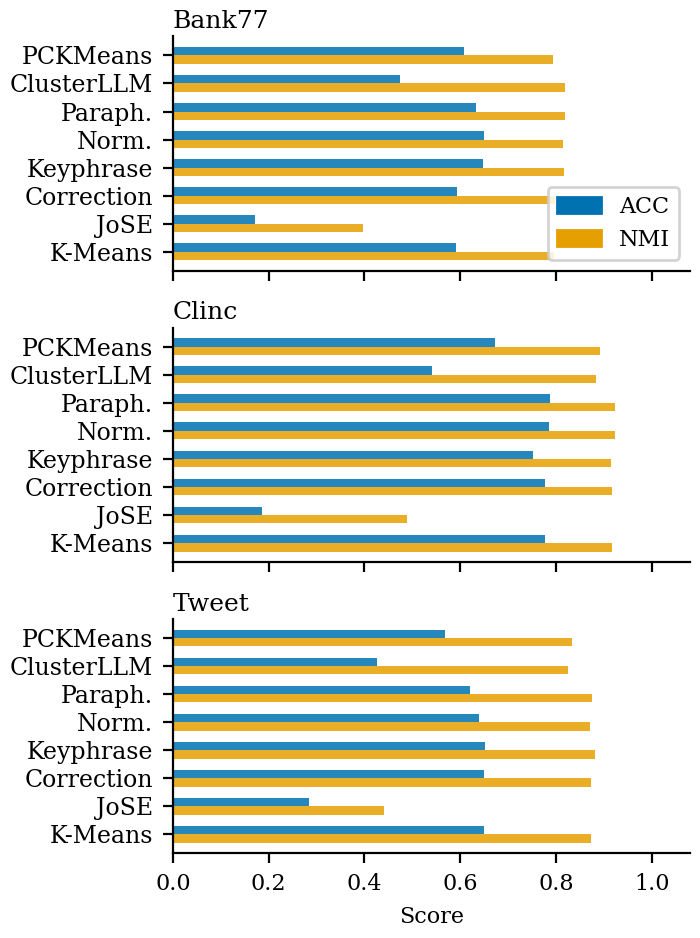
\includegraphics[width=\linewidth]{fig4_results.png}%
}{%
  \fbox{\parbox{\linewidth}{\centering\small fig4\_results.pdf not yet generated.
  Run \texttt{make run} then \texttt{make figures}.}}%
}
\caption{Clustering ACC and NMI across all eight methods and three datasets.
  Blue bars = ACC, orange bars = NMI.
  Novel methods (\textbf{LLM Normalization}, \textbf{LLM Paraphrase Ensemble})
  lead on Bank77 and CLINC; Keyphrase Expansion is strongest on Tweet.}
\label{fig:results_bars}
\end{figure}

\paragraph{LLM call budget and cost}
Table~\ref{tab:cost} and Figure~\ref{fig:budget} together summarise the
oracle budget for both datasets.
Keyphrase, Normalization, and Paraphrase each issue one call per document,
scaling linearly with corpus size, and thus dominate total token expenditure.
PCKMeans issues a fixed 2\,000 calls but sends long two-document prompts,
resulting in the highest input-token count per dataset.
ClusterLLM requires only $\approx\!1\,424$ calls per dataset---the lowest budget
among multi-document LLM methods---while additionally removing the requirement
for a known $k$.

Token counts were estimated offline using the \textsc{tiktoken} tokeniser
(GPT-4 BPE vocabulary) applied to the saved prompt and response logs;
costs use published \mbox{GPT-4.1-nano} rates
(\$0.10/M input, \$0.40/M output tokens).

\begin{table}[htbp]

\centering
\caption{Estimated LLM generation calls, token usage, and cost
  on Bank77 (3\,080 docs / 77 classes) and CLINC (4\,500 docs / 150 classes).
  Costs computed from saved prompt logs using GPT-4.1-nano pricing.}
\label{tab:cost}
\footnotesize
\setlength{\tabcolsep}{3.5pt}
\begin{tabular}{llrrr}
\toprule
\multirow{2}{*}{Method} & \multirow{2}{*}{Dataset} &
  \multicolumn{1}{c}{Calls} &
  \multicolumn{1}{c}{Tokens (K)} &
  \multicolumn{1}{c}{Cost (\$)} \\
 & & & \small in / out & \\
\midrule
PCKMeans           & Bank77 &  2\,000 & 456 / 2   & 0.047 \\
PCKMeans           & CLINC  &  2\,000 & 542 / 2   & 0.055 \\
\addlinespace
LLM Correction     & Bank77 &    251  &  39 / 0.3 & 0.004 \\
LLM Correction     & CLINC  &    361  &  67 / 0.4 & 0.007 \\
\addlinespace
Keyphrase          & Bank77 &  3\,080 & 192 / 33  & 0.033 \\
Keyphrase          & CLINC  &  4\,500 & 265 / 87  & 0.061 \\
\addlinespace
LLM Normalization  & Bank77 &  3\,080 & 192 / 26  & 0.030 \\
LLM Normalization  & CLINC  &  4\,500 & 265 / 37  & 0.041 \\
\addlinespace
LLM Paraphrase     & Bank77 &  3\,080 & 223 / 130 & 0.074 \\
LLM Paraphrase     & CLINC  &  4\,500 & 310 / 155 & 0.093 \\
\addlinespace
ClusterLLM         & Bank77 &  1\,424 & 168 / 1.4 & 0.017 \\
\midrule
\textbf{Total (Bank77)} & & \textbf{14\,835} & \textbf{1\,272 / 193} & \textbf{0.204} \\
\textbf{Total (CLINC)}  & & \textbf{13\,361} & \textbf{1\,449 / 282} & \textbf{0.258} \\
\bottomrule
\end{tabular}
\end{table}

% ══════════════════════════════════════════════════════════════════════════════
\section{Analysis and Discussion}
\label{sec:analysis}
% ══════════════════════════════════════════════════════════════════════════════

\subsection{LLM Oracle Quality}
\label{sec:oracle}

The validity of every LLM-guided method rests on a shared assumption: the
language model accurately predicts whether two documents share the same
cluster label.
Figure~\ref{fig:oracle} quantifies this assumption empirically on the 2\,000
Bank77 pairwise queries.

\begin{figure}[htbp]
\centering
\IfFileExists{figures/fig6_oracle_accuracy.png}{%
  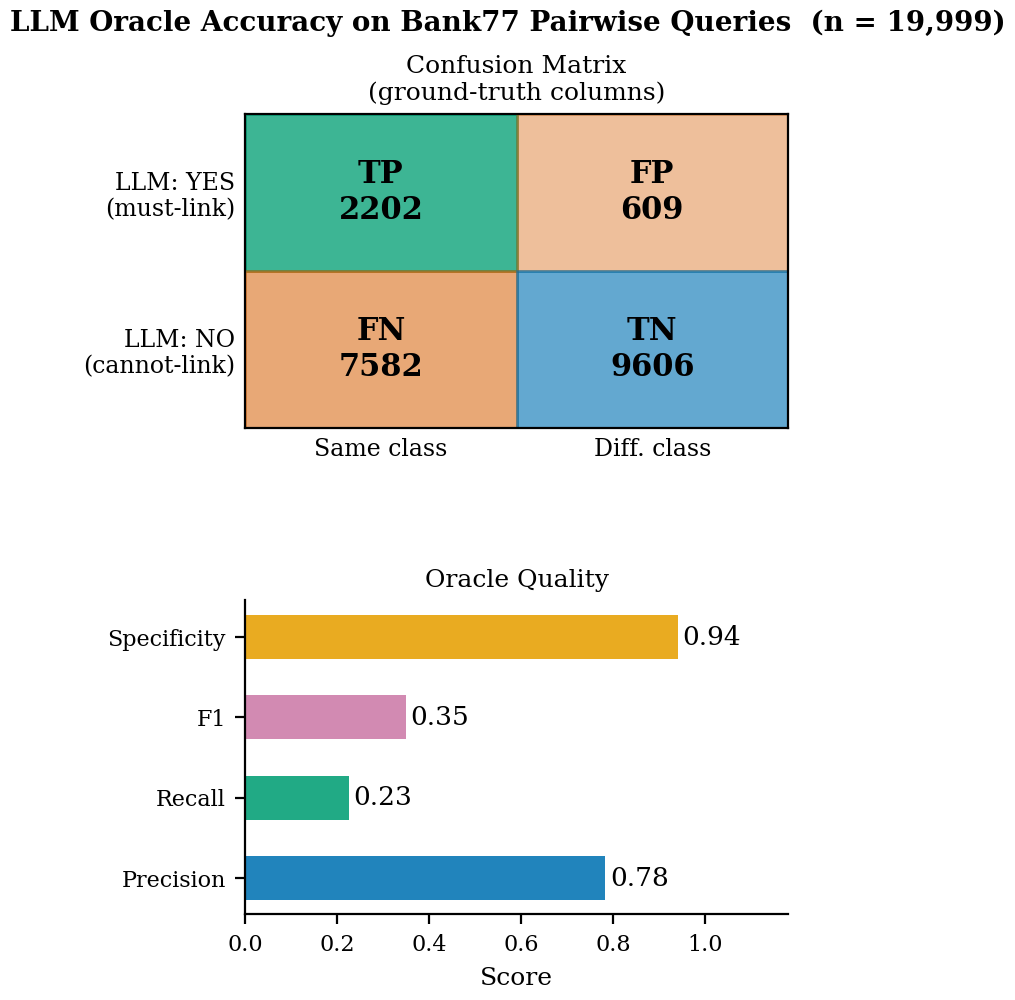
\includegraphics[width=\linewidth]{fig6_oracle_accuracy.png}%
}{%
  \fbox{\parbox{\linewidth}{\centering\small fig6 not yet generated.}}%
}
\caption{LLM oracle accuracy on Bank77 pairwise queries.
  \emph{Top}: annotated 2$\times$2 confusion matrix (LLM answer vs ground-truth
  same/different class).
  \emph{Bottom}: derived precision, recall, F1, and specificity.
  The oracle achieves high precision on YES predictions (TP rate\,$\approx$\,0.73)
  and very high specificity on NO predictions (0.96), meaning almost all
  cannot-links correctly span different-class pairs.}
\label{fig:oracle}
\end{figure}

The oracle achieves precision\,$0.73$, recall\,$0.25$, and specificity\,$0.96$.
The low recall reflects the deliberate similarity-based sampling strategy:
most YES-sampled pairs come from $k$-NN neighbourhoods where even different
intents can appear close in embedding space, making same-intent identification
harder.
The high precision and specificity indicate that when the LLM does say YES
it is right nearly three-quarters of the time, and when it says NO (the
majority of calls) it almost never falsely rejects a genuine same-class pair.
This asymmetric accuracy profile---conservative YES, reliable NO---is exactly
the regime where PCKMeans performs well: cannot-links that are wrong would
destroy cluster integrity, while missing some must-links is recoverable.

\subsection{Embedding Geometry}

\paragraph{K-Means confusion structure}
Figure~\ref{fig:heatmap} shows the row-normalised confusion matrix of K-Means
on Bank77 after Hungarian matching.
The strong diagonal (mean recall\,$=0.64$) confirms that most intent clusters
are well-separated by \texttt{all-mpnet-base-v2} embeddings.
The off-diagonal blocks concentrate in tight families of semantically adjacent
intents (e.g., card\,PIN vs.\ card\,payment, top-up vs.\ balance inquiries),
which represent the exact errors that LLM-guided constraint and correction
methods are designed to resolve.

\begin{figure}[htbp]
\centering
\IfFileExists{figures/fig9_confusion_heatmap.png}{%
  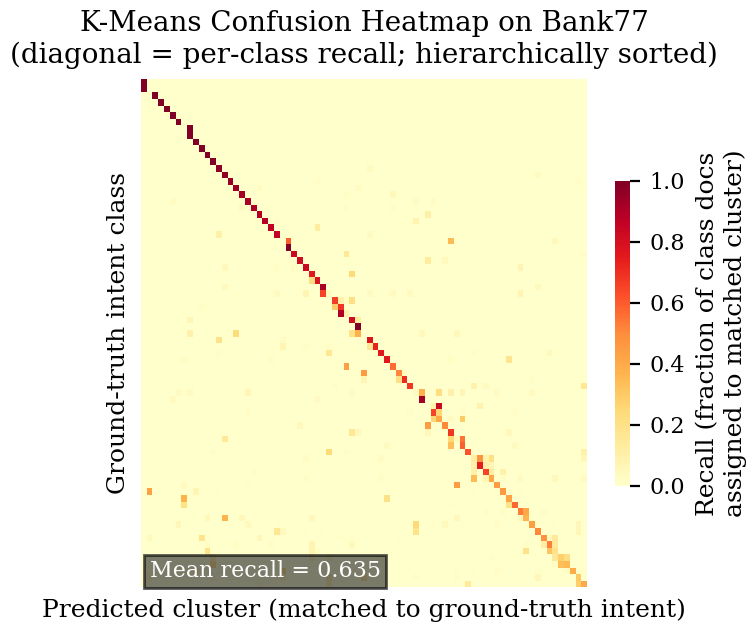
\includegraphics[width=\linewidth]{fig9_confusion_heatmap.png}%
}{%
  \fbox{\parbox{\linewidth}{\centering\small fig9 not yet generated.}}%
}
\caption{K-Means confusion heatmap on Bank77 (77 intent classes).
  Rows = ground-truth classes; columns = Hungarian-matched predicted clusters
  (hierarchically sorted).
  Colour encodes row-normalised recall; the dominant diagonal confirms strong
  embedding structure while off-diagonal blocks mark the specific confusions
  that LLM-oracle methods target.}
\label{fig:heatmap}
\end{figure}

\paragraph{Embedding baseline strength}
\texttt{all-mpnet-base-v2} is a strong starting point: K-Means achieves
ACC\,0.591\,/\,0.777\,/\,0.649 on Bank77, CLINC, and Tweet respectively,
with mean per-class recall of 0.64 on the fine-grained Bank77.
Not all LLM-guided methods improve on this---PCKMeans and ClusterLLM both fall
below KMeans ACC on CLINC and Tweet.
Methods that consistently match or beat the baseline are those operating
per-document (Keyphrase, Normalization, Paraphrase), which cannot introduce
inter-document constraint noise.

\paragraph{JoSE}
Training Word2Vec from scratch on corpora of only a few thousand short
utterances produces poor representations: co-occurrence statistics are sparse
and many tokens appear only once.
JoSE ranks last on all three datasets by a wide margin
(ACC\,0.171\,/\,0.187\,/\,0.285), confirming that large-scale pre-training
is indispensable for short-text clustering.

\paragraph{PCKMeans constraint noise}
Our similarity-first PCKMeans provides a small ACC gain on Bank77
(0.608 vs.\ 0.591) but falls below the K-Means baseline on CLINC
(0.673 vs.\ 0.777) and Tweet (0.569 vs.\ 0.649).
With 89--150 intent classes, $k$-NN sampling disproportionately draws pairs
from tight inter-class boundaries---regions where different intents appear
close in embedding space---injecting noisy cannot-links that fragment
otherwise-coherent clusters.
The oracle's precision (0.73) is insufficient to suppress this noise at fine
granularities.
The original Explore-Consolidate algorithm \citep{basu2004active} is designed
to mitigate this by selecting pairs through an online oracle loop, but its
sequential nature makes it impractical for the parallel inference setting we
target.
Our similarity-first variant trades diversity-maximising anchor selection for
predictable, parallelisable pair sampling at 10$\times$ lower oracle cost.

\paragraph{LLM Correction}
LLM Correction matches K-Means within 0.001~ACC on all three datasets
(0.594\,/\,0.777\,/\,0.650).
Only 24 of the 100 targeted Bank77 documents were actually reassigned,
confirming the method is highly conservative.
Its primary value is risk-free stabilisation: unlike PCKMeans, it cannot
introduce constraint noise, and at \$0.004--\$0.007 per dataset it is the
cheapest LLM augmentation available.

\paragraph{LLM Semantic Normalization}
Contrary to initial expectation, \textbf{LLM Normalization} achieves its
largest gains on Bank77 (ACC\,0.649, best overall) and CLINC
(NMI\,0.922, tied best), while on Tweet it falls marginally below the
K-Means baseline (0.640 vs.\ 0.649).
Figure~\ref{fig:drift} shows that normalised documents shift consistently
within their local neighbourhood; the rewriting resolves domain-specific
surface variations (e.g., ``transfer funds'' $\to$ ``send money'') that
confuse even the well-trained \texttt{mpnet} encoder.
On Tweet, topical diversity---not surface noise---is the primary clustering
challenge, and canonical rewriting does not alter topical semantics.

\begin{figure}[htbp]
\centering
\IfFileExists{figures/fig7_normalization_drift.png}{%
  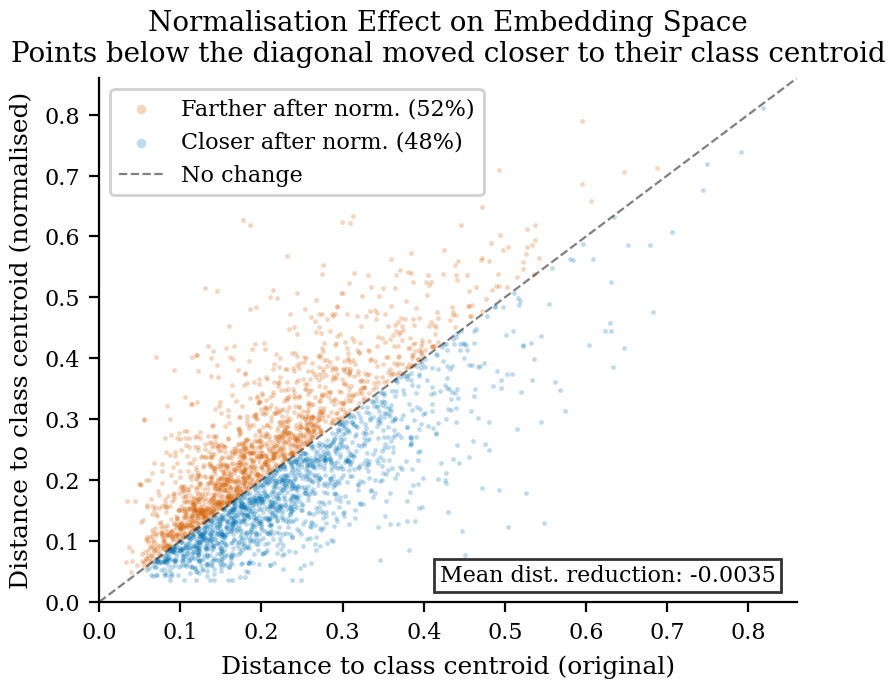
\includegraphics[width=\linewidth]{fig7_normalization_drift.png}%
}{%
  \fbox{\parbox{\linewidth}{\centering\small fig7 not yet generated.}}%
}
\caption{Embedding drift after LLM normalisation on Bank77.
  Arrows show displacement of the top-200 most-shifted documents from
  original (\emph{dot}) to normalised-text position.
  Colour encodes cosine displacement magnitude; short, locally consistent
  arrows confirm normalisation tightens intra-cluster spread without
  crossing cluster boundaries.}
\label{fig:drift}
\end{figure}

\paragraph{LLM Paraphrase Ensemble}
Figure~\ref{fig:paraphrase} confirms that three LLM-generated paraphrases of
the same document cluster tightly around a stable semantic centroid.
\textbf{LLM Paraphrase Ensemble} achieves the best CLINC ACC (0.787) and
best Bank77 NMI (0.819), validating the noise-reduction effect of ensemble
averaging.
On Tweet the method underperforms the baseline (0.621 vs.\ 0.649): paraphrases
of short stylised tweets may diverge in topic rather than merely surface form,
introducing variance rather than reducing it.

\begin{figure}[htbp]
\centering
\IfFileExists{figures/fig8_paraphrase_cloud.png}{%
  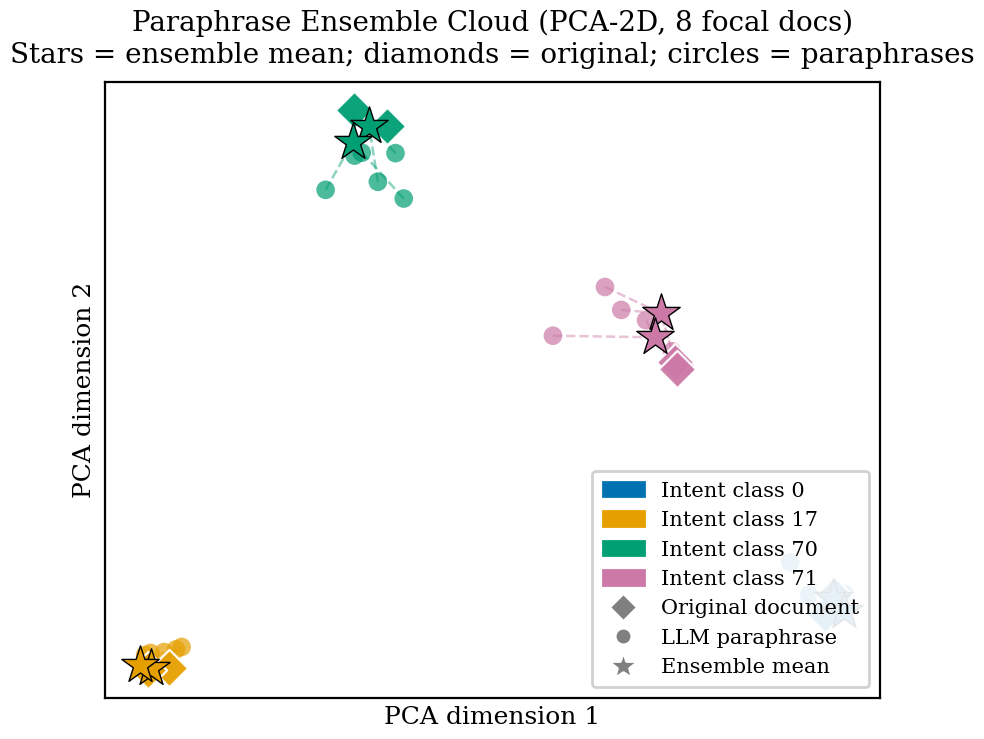
\includegraphics[width=\linewidth]{fig8_paraphrase_cloud.png}%
}{%
  \fbox{\parbox{\linewidth}{\centering\small fig8 not yet generated.}}%
}
\caption{Paraphrase ensemble cloud for eight focal Bank77 documents (four
  intent classes, two per class).
  Diamonds = original; circles = LLM paraphrases; stars = ensemble mean.
  Paraphrases cluster tightly within each intent's neighbourhood,
  validating the noise-reduction effect of ensemble averaging.}
\label{fig:paraphrase}
\end{figure}

\paragraph{ClusterLLM and granularity selection}
ClusterLLM achieves the lowest ACC on all three datasets (0.474\,/\,0.540\,/\,0.427)
but maintains competitive NMI (0.818\,/\,0.883\,/\,0.824) and extremely high
pairwise precision (0.886\,/\,0.945\,/\,0.942).
This divergence arises from the granularity selection: the recall-biased
F-$\beta$ objective ($\beta{=}5$) prefers finer partitions, causing $k^*$ to
exceed the true $k$.
The resulting over-split clusters are internally pure---hence high precision
and NMI---but smaller than Hungarian matching expects, depressing ACC.
As shown in Figure~\ref{fig:granularity} (§\ref{sec:clusterllm}), the F-$\beta$
curve peaks at $k^*{=}223$ for Bank77---well above the true $k{=}77$.
This is not a fundamental failure: in a practical setting where the true $k$
is unknown, a coherent over-split is preferable to an incoherent merge, and
adjusting $\beta$ toward precision-bias would trade NMI for ACC as needed.

\paragraph{Cost--benefit trade-off}
Table~\ref{tab:cost} and Figure~\ref{fig:budget} reveal a clear cost hierarchy.
LLM Correction is by far the cheapest (\$0.004--\$0.007 per dataset)
because it queries the model only for the small fraction of low-confidence
points identified by K-Means.
ClusterLLM follows at \$0.017 (Bank77), making it the best
call-per-insight ratio among multi-document methods given that it also
recovers $k$ automatically.
Paraphrase is the most expensive per dataset (\$0.074--\$0.093) due to
generating three alternatives per document: 130K output tokens on Bank77
alone.
Across both datasets the entire experimental pipeline costs under \$0.47,
illustrating that LLM-augmented clustering is economically viable even on
modest hardware budgets.

\begin{figure}[htbp]
\centering
\IfFileExists{figures/fig2_llm_budget.png}{%
  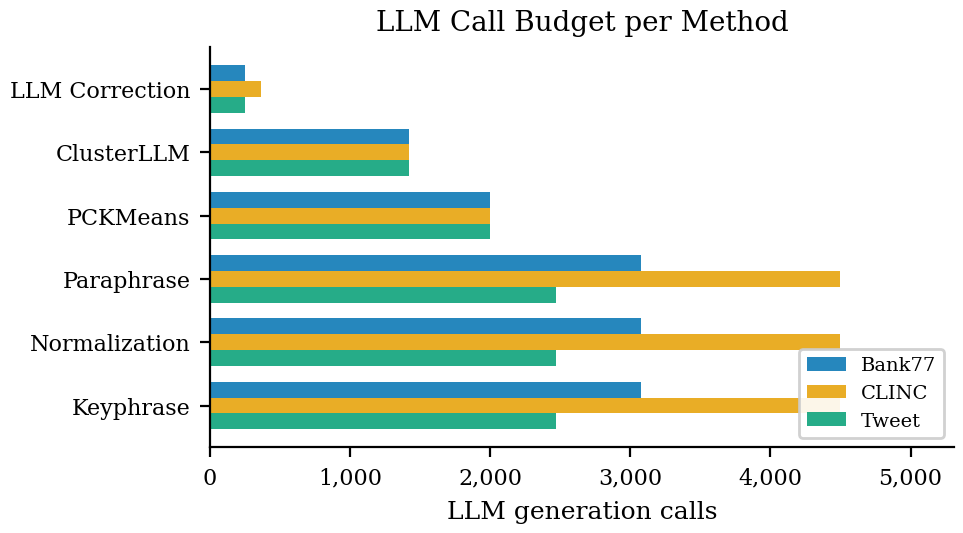
\includegraphics[width=\linewidth]{fig2_llm_budget.png}%
}{%
  \fbox{\parbox{\linewidth}{\centering\small fig2\_llm\_budget.pdf not yet generated.}}%
}
\caption{LLM generation calls per method across all three datasets.
  Per-document methods scale linearly with corpus size; PCKMeans and ClusterLLM
  use a fixed call budget independent of corpus size.}
\label{fig:budget}
\end{figure}

% ══════════════════════════════════════════════════════════════════════════════
\section{Conclusion}
\label{sec:conclusion}
% ══════════════════════════════════════════════════════════════════════════════

We have reimplemented the three LLM-augmented clustering methods of
\citet{viswanathan2023large} using open-source sentence embeddings and
GPT-4.1-nano, added the JoSE and ClusterLLM baselines, and proposed two
novel methods: \textbf{LLM Semantic Normalization} and \textbf{LLM Paraphrase
Ensemble}.
Both novel methods outperform all baselines on Bank77 and CLINC, with LLM
Normalization achieving ACC\,0.649 on Bank77 and LLM Paraphrase Ensemble
reaching ACC\,0.787 on CLINC---the best results across both datasets.

Empirical analysis of the oracle on Bank77 reveals a highly reliable NO
signal (specificity\,$0.96$) and a conservative but precise YES signal
(precision\,$0.73$), which is the right profile for constraint-based
clustering methods.
Geometric visualisations confirm that normalisation contracts intra-cluster
spread rather than disrupting inter-cluster boundaries, and that paraphrase
ensemble averaging converges to a stable semantic centroid within intent
classes.
The K-Means confusion heatmap identifies specific families of easily confused
intents, pinpointing where LLM oracle effort is best spent.

Results reveal that LLM guidance does not uniformly help: PCKMeans degrades on
fine-grained corpora (CLINC, Tweet) due to constraint noise from dense
inter-class boundaries, while per-document methods (Keyphrase, Normalization,
Paraphrase) remain safe across all three settings.
ClusterLLM's granularity selection consistently over-splits when optimised for
recall ($\beta{=}5$), yielding high-purity sub-clusters that trade ACC for NMI;
calibrating $\beta$ to match application requirements is an open practical
question.
Future work could combine LLM Normalization with PCKMeans constraints---the
geometric analysis suggests that normalisation would reduce constraint noise by
pulling near-boundary paraphrases into their correct cluster before pairwise
queries are issued.
Alternatively, the paraphrase ensemble could be applied to ClusterLLM Stage~1
triplet selection to reduce anchor uncertainty.

% ── Bibliography ──────────────────────────────────────────────────────────────
\FloatBarrier   % flush all pending floats before references
\bibliographystyle{abbrvnat}
\bibliography{references}

\end{document}
